% Chapter Template

\chapter{Introduction REPTAR} % Main chapter title

\label{Chapitre 2} % Change X to a consecutive number; for referencing this chapter elsewhere, use \ref{ChapterX}

\lhead{ \emph{Introduction REPTAR}} % Change X to a consecutive number; this is for the header on each page - perhaps a shortened title

%----------------------------------------------------------------------------------------
%	SECTION 1
%----------------------------------------------------------------------------------------
\section{Manipulations}

Comme mentionné dans la donnée du laboratoire, les sous chapitres suivant vont présenter le résultat des manipulations effectuée en groupe de deux.

\subsection{Manipulation 5}
Le but de cette manipulation est de déployer une application simple qui fonctionne premièrement dans U-Boot, et ensuite dans Linux.\\

Voici les manipluation effectuée pour le déployement dans U-Boot :
\begin{enumerate}
\item Compiler le projet "helloworld\_uboot" dans eclipse.
\item Copier le fichier "helloworld.bin", résultat de la compilation, dans le dossier /home/redsuser/tftpboot (pour avoir accès depuis le serveur de fichier)
\item Dans U-Boot, faire la commande suivante : "setenv appExample tftp 0x81600000 helloworld.bin". Cela nous permet de copier le binaire en mémoire à l'adresse 0x81600000.
\item Dans U-Boot, faire la commande suivante : "run appExample". Cela nous permet de lancer la copie, comme expliqué précédemment.
\item Dans U-Boot, faire la commande suivante : "go 0x81600000". Cela nous permet de lancer l'application.\\
\end{enumerate}

Voici ci-dessous le résultat obtenu de l'exécution : 

\begin{center} 
\hspace{12.45cm}
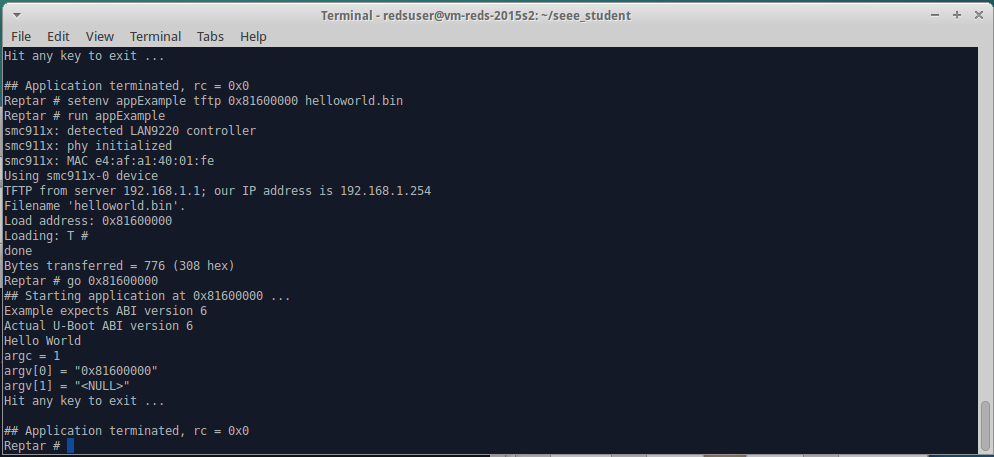
\includegraphics[width=15cm]{uboot_hello_result.png}
\end{center}
\vspace{1cm} 

\pagebreak

Voici les manipluation effectuée pour le déployement dans Linux :
\begin{enumerate}
\item Compiler le projet "helloworld\_linux" dans eclipse.
\item Insérer la carte SD dans la carte REPTAR (après l'avoir correctement alimentée), afin de "booter" sur linux.
\item Depuis la cible, nous allons utiliser la commande "scp" pour télécharger le fichier "helloworld" par "ssh" sur la machine de développement.
\end{enumerate}

Voici le résultat de la commande "scp", ainsi que l'exécution du programme sur la cible : 

\begin{center} 
\hspace{12.45cm}
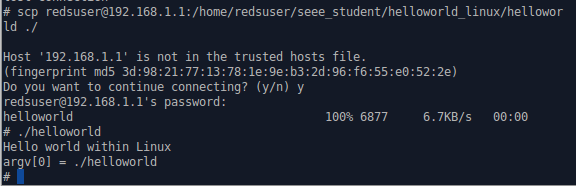
\includegraphics[width=15cm]{linux_scp.png}
\end{center}
\vspace{1cm} 

\pagebreak
\subsection{Manipulation 6}

